\subsection{Sprint 2}

\subsubsection{Introduction}

\subsubsection{UMLs}

In this Sprint 2, we have started on the initial implementation of the bridge and design of UML for Pacman.

\subsubsection{UMLs}

At this point, we have started with our next game which was Pacman, so the we designed an UML for it

\begin{itemize}
    \item Task ID - 72: \href{https://github.com/Pending-Name-21/arquitecture/pull/11}{Pacman UML Diagram on GitHub}
\end{itemize}

\subsubsection{Spikes}

There were no Spikes

\subsubsection{POCs}

In this Sprint, we had no Proofs of Concept (POCs).

\subsubsection{Technical Justification}

During Sprint 2, the team focused on designing UMLs of the games
and start on the initial phase of the brigde. This decision was based on the following reasons:

\subsubsection{High - Level Architecture}

The architecture followed in this sprint was based on the initial architecture.

\begin{itemize}
    \item Architecture: \href{https://github.com/Pending-Name-21/arquitecture/pull/1/files}{Architecture Initial Version}
    You can see it on: 
    \item C4 DSL: \href{https://structurizr.com/dsl}{Visualizer}
\end{itemize}

\subsubsection{Impediments}
\href{https://docs.google.com/spreadsheets/d/1ty_hOe11I5BHMMoJYUfMxHD2sC9OoST2Nor8Q2Cqvq0/edit?usp=sharing}{impediments}

\subsubsection{Epics}
For this Sprint 2, we have the following epics:

\begin{itemize}
    \item Bridge
    \item Console
    \item Graphics
    \item Games
\end{itemize}

\PassOptionsToPackage{unicode}{hyperref}
\PassOptionsToPackage{hyphens}{url}
\documentclass{article}
\setcounter{secnumdepth}{3}

\usepackage{amsmath,amssymb}
\usepackage{lmodern}
\usepackage{iftex}
\usepackage[letterpaper, margin=1in, top=0.5in, bottom=1in]{geometry}
\usepackage{listings}
\usepackage{color}
\usepackage{titling}
\usepackage{graphicx}
\usepackage{hyperref}

\ifPDFTeX
  \usepackage[T1]{fontenc}
  \usepackage[utf8]{inputenc}
  \usepackage{textcomp} 
\else 
  \usepackage{unicode-math}
  \defaultfontfeatures{Scale=MatchLowercase}
  \defaultfontfeatures[\rmfamily]{Ligatures=TeX,Scale=1}
\fi
\IfFileExists{upquote.sty}{\usepackage{upquote}}{}
\IfFileExists{microtype.sty}{
  \usepackage[]{microtype}
  \UseMicrotypeSet[protrusion]{basicmath} 
}{}
\makeatletter
\@ifundefined{KOMAClassName}{
  \IfFileExists{parskip.sty}{
    \usepackage{parskip}
  }{
    \setlength{\parindent}{0pt}
    \setlength{\parskip}{6pt plus 2pt 2pt}}
}{
  \KOMAoptions{parskip=half}}
\makeatother
\usepackage{xcolor}
\usepackage{graphicx}

\makeatletter
\def\maxwidth{\ifdim\Gin@nat@width>\linewidth\linewidth\else\Gin@nat@width\fi}
\def\maxheight{\ifdim\Gin@nat@height>\textheight\textheight\else\Gin@nat@height\fi}
\makeatother
\setkeys{Gin}{width=\maxwidth,height=\maxheight,keepaspectratio}
\makeatletter
\def\fps@figure{htbp}
\makeatother
\setlength{\emergencystretch}{3em} 
\providecommand{\tightlist}{
  \setlength{\itemsep}{0pt}\setlength{\parskip}{0pt}}

\ifLuaTeX
  \usepackage{selnolig}  
\fi
\IfFileExists{bookmark.sty}{\usepackage{bookmark}}{\usepackage{hyperref}}
\IfFileExists{xurl.sty}{\usepackage{xurl}}{} 
\urlstyle{same}
\hypersetup{
  hidelinks,
  pdfcreator={LaTeX via pandoc}}

\title{Artifacts - Sprint 2}
\date{}

\begin{document}

\maketitle

\hypertarget{burndownchart-s2}{
\section{Burn Down Chart}\label{Burn Down Chart S2}}
\href{https://tree.taiga.io/project/joseluis-teran-coffeetime/taskboard/sprint-2-12274}{Link: Sprint 2 Board on Taiga}.

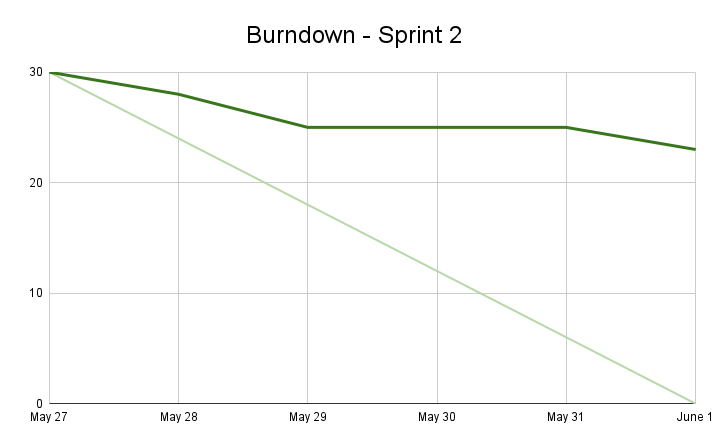
\includegraphics[width=\textwidth]{./assets/Burndown - Sprint 2.png}

\hypertarget{startstopcontinueactionitems-s2}{
\section{Start-Stop-Continue-Action Items}\label{Start-Stop-Continue-Action Items S2}}
\href{https://miro.com/app/board/uXjVKDO7l8M=/?moveToWidget=3458764590247693277&cot=14}{Link: Start-Stop-Continue-Action Items Sprint 2 on Miro}.

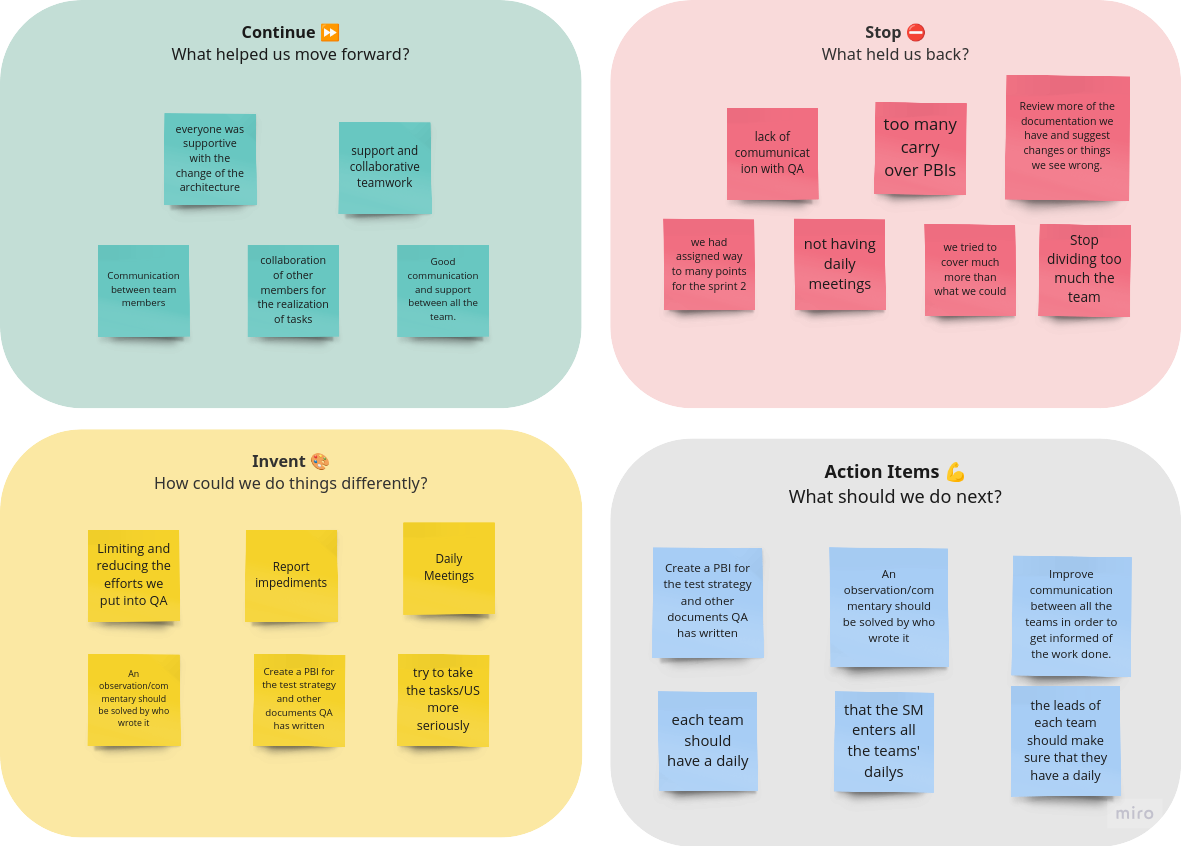
\includegraphics[width=\textwidth]{./assets/retrospective-s2.png}

\end{document}

\subsubsection{Backlog - Sprint 2}

\subsubsection*{Task Board}
\href{https://tree.taiga.io/project/joseluis-teran-coffeetime/taskboard/sprint-2-12274}{Sprint 2 Task Board}

\subsubsection*{Completed User Stories}

\begin{enumerate}
    \item \textbf{71 Pacman Mockups and Sprites} \\
    \textit{Assigned to:} Sebastian Barra \\
    \textit{Status:} Done in Sprint
    \item \textbf{18 UML: Library} \\
    \textit{Assigned to:} Santiago Concha (carryover from last sprint) \\
    \textit{Status:} Done in Sprint
    \item \textbf{19 Spike: Graphics Libraries for Console} \\
    \textit{Assigned to:} Jose Luis Teran (carryover from last sprint)\\
    \textit{Status:} Done in Sprint
    \item \textbf{20 Spike: Console with JNI} \\
    \textit{Assigned to:} Fabian Romero(carryover from last sprint)\\
    \textit{Status:} Done in Sprint
    \item \textbf{64 Input Management} \\
    \textit{Assigned to:} Luiggy Mamani and Axel Ayala \\
    \textit{Status:} Done in Sprint
    \item \textbf{91 Sound Management} \\
    \textit{Assigned to:} Alex Paca \\
    \textit{Status:} Done in Sprint
    \item \textbf{76 Input Handler for the Bridge} \\
    \textit{Assigned to:} Gabriel Concha and Fabian Romero \\
    \textit{Status:} Done in Sprint
    \item \textbf{107 Update Handler} \\
    \textit{Assigned to:} Gabriel Concha and Fabian Romero \\
    \textit{Status:} Done in Sprint
    \item \textbf{114 QA - Test Cases for Games} \\
    \textit{Assigned to:} Josue Prado and Luis Espinoza \\
    \textit{Status:} Done in Sprint
\end{enumerate}

\subsubsection*{Carryover User Stories}

\begin{enumerate}
    \item \textbf{88 Implementation of Render Handler} \\
    \textit{Assigned to:} Fabian Romero and Sebastian Sebastian Barra\\
    \textit{Status:} Carryover
    \item \textbf{72 Pacman UML} \\
    \textit{Assigned to:} Victor Villca, Jhael Arce and Ronaldo Mendoza \\
    \textit{Status:} Carryover
\end{enumerate}


\subsubsection{Conclusions}

In Sprint 2, we started to work on the basics but unfortunately 
we could not finish so the user stories were moved to carry over 
but they helped us to see the beginning of the work ahead of us.
